\documentclass[conference]{IEEEtran}
\usepackage[utf8]{inputenc}
\usepackage{cite}
\usepackage{amsmath,amssymb,amsfonts}
\usepackage{algorithmic}
\usepackage{graphicx}
\usepackage{textcomp}

\title{Design a block chain enabled time banking web application}

\author{
\IEEEauthorblockN{Xuheng Lin, Ronghua Xu, Yu Chen}
\IEEEauthorblockA{%\textit{Dept. of Electrical \& Computer Engineering} \\
Dept. of Electrical and Computer Engineering, Binghamton University, SUNY, Binghamton, NY 13902, USA \\
\{rxu22, xlin84, ychen\}@binghamton.edu}
}
%\date{October 2018}

\begin{document}

\maketitle

\begin{abstract}


\end{abstract}

\begin{IEEEkeywords}
Blockchain, Smart Contract, Time Banking.
\end{IEEEkeywords}



\section{Introduction}
The block chain technology provides a more secure way of making transaction due to its decentralized characteristics and consensus mechanism. Every transaction becomes more transparency than ever before. And the consensus mechanism encourages people to get involved in this prosperous decentralized network. While, smart contract guarantees that the agreement is immutable and unbroken. People can rely on these to avoid being cheated. Thanks to such characteristics, many p2p web applications can be built based on block chain and smart contract, for example, time banking. 

Time Banking is a generalized exchange economy not based on money, and values everyone’s contribution on the same scale (time expended) \cite{carroll2013co}. Time banking has spread rapidly in recent years; for example, the nonprofit organization, TimeBanks USA \cite{TimeBanksUSA} facilitates 276 time banks in North America through 27,000 members, as well as in other countries. In time banking system, all members’ time is treated as equal, which allows value created by service exchanges to remain within the local community. Apart from the obvious benefit of allowing people without money or a job to participate in value creation, a time bank creates opportunities for new relationships to form and strengthens bonds among community members \cite{bellotti2014towards}. Time banking itself is also a network, which functions as a platform letting people provide and receive services from each other by donate their time. Generally, it does not involve real money. One simple example is that one person can hire another one for massaging for one hour. Then, the masseur earns one hour credits and next time, the masseur can spend the credits to hire other people to work for him/her for one hour.

There are five core values of time banking as listed by Edgar Cahn, the founder of modern time banking \cite{cahn2011time}, \cite{cahn2000no}.

\begin{itemize}
   \item First, the asset, everyone has something to provide, from washing dishes to taking care of elder people, or even providing accompanying. 
   \item Second, redefining work, some work cannot be found on the market like revitalizing neighborhoods, or is hard to hire someone who is trust worthy. 
   \item Third, reciprocity, this emphasis providing and receiving among the neighbors and thus helps building strong connections between neighborhoods. 
   \item Fourth, social networks, it will be strengthened by time banking because time banking provides a way that allows people to share their skills among each other. 
   \item Fifth, respect, every transaction in the time banking is based on the agreement and trust. And because block chain is enabled in time banking thus the trust can be guaranteed. 
 \end{itemize}

 %Fig2_time_banking
\begin{figure} [t]
\begin{center}
\begin{tabular}{c}
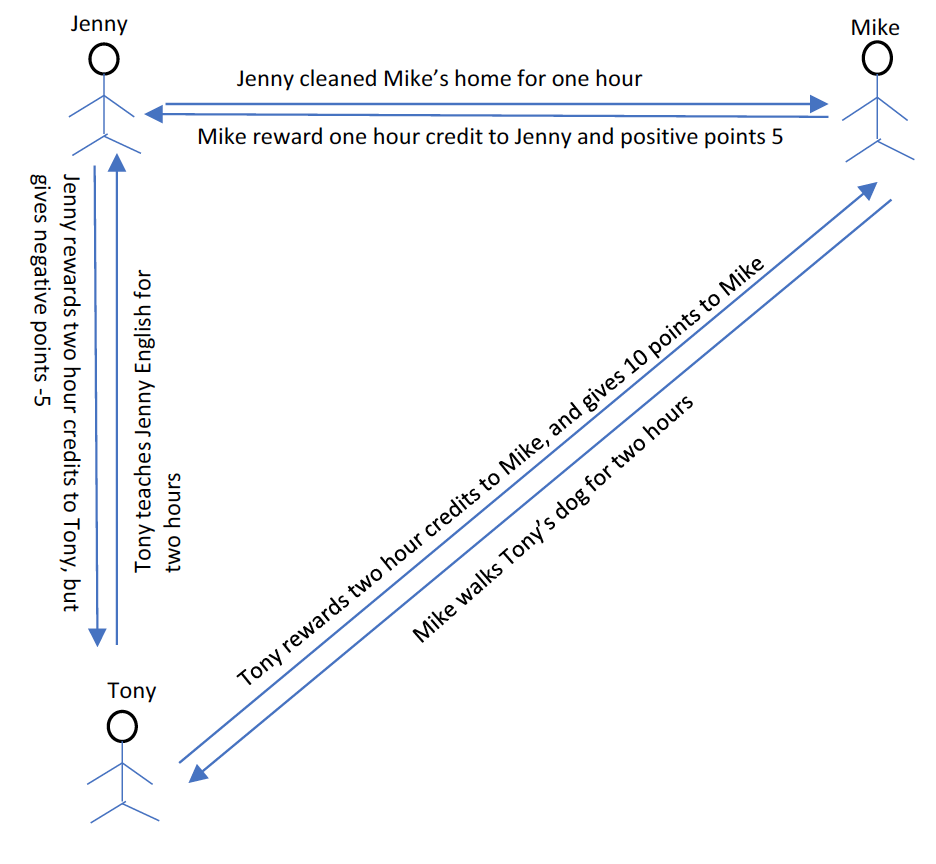
\includegraphics[height=7.5cm]{time_bank_picture}
\end{tabular}
\end{center}
\caption[example] {\label{fig:1-time banking} Illustration of time banking system.}
\vspace{-10pt}
\end{figure}

\section{system design}
 Different from traditional web applications that relies heavily on a central server, block chain enabled time banking application uses the Ethereum platform to achieve it's goal of a decentralized application. 

 First, a group of users will be created with unique public key and certain hours for development purpose. The public key is used to identify each of them in the system, and the hours is users' initial deposit which can be spent to receive service from others.  Than a smart contract defining the transaction, which is between the time and service, is made among these users. 
 
 The smart contract plays an important role in the application. A smart contract is a computer protocol intended to digitally facilitate, verify, or enforce the negotiation or performance of a contract.\cite{wiki} In the contract, some rules will be defined in order to pass the transaction, like the basic line of a user's credit score. If a user doesn't have enough credit score, than this user may need to do some volunteer work to increase the credits.   
 
The user can offer and request services in the time banking. These services will be uploaded to the contract and be recorded in the block chain. All the services provided by each user will be shown to the front end. When a user wants to receive the service provided by another one, this user can apply for that service. After the amplification, the information of the applier will filtered by the smart contract. The information may including credits score, social background and so on. If the information passed the contract criteria, the applier will be ready to receive the service but has to wait until the service provider finish the same filtering process. Such process ensures that the transaction is safe because users may not know each other until their first meet and the contract eliminates their worries.

\section{future work}
The block chain enabled time banking would have a huge impact in a few years later. Because people can enjoy services without spending money and community relationship really strengthened, especially for the elder and low income people, who need social care most. As more and more people involve in the time banking in the future,   


 
\bibliographystyle{IEEEtranS}
\bibliography{timebanking}
\end{document}
